\section{Genetic Algorithm}
\label{sec:ga}

A genetic algorithm (GA) is a search heuristic that mimics natural selection. In a GA individuals go through a \textit{selection} process and are bred(\textit{crossed}) with other individuals to create new individuals. Individuals in a GA are commonly refered to as \textit{chromosomes}. Figure~\ref{fig:gaFlowchart} depicts how evolution occurs in a GA.

\begin{figure}[H]
  \centering
  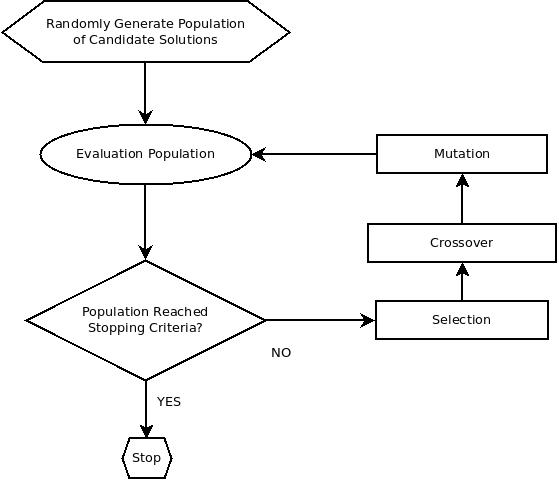
\includegraphics[bb=0 0 288 390,scale=0.5]{figures/GA.jpeg}
  \caption{GA Evolution}
  \label{fig:gaFlowchart}
\end{figure}

During each generation a new population is created using the previous generation's population. Initially the best individuals from the previous population might be copied directly into the new population using an operator called \textit{elitism}. To obtain the remaining individuals needed to fill the new population a \textit{selection} process occurs. Two individuals are chosen using a \textit{selection} method and then one of three options can occur: \textit{crossover}, \textit{mutation}, or \textit{replication}. Crossover mixes two individuals together to create two new individuals, mutation randomly modifies each individual individually, and replication copies the individuals. The two individuals are then placed in the new population and the process is repeated until the new population is the same size as the previous population. Figure~\ref{fig:gaFlowchart} depicts how evolution occurs in a GA. See Subsection~\ref{subsec:ga-operators} for more details on the operators discussed.

\subsection{Chromosome}

The individuals of a GA represent possible candidate solutions to the problem. Typically a chromosome is represented as an array where each index of the array represents a property of the candidate solution. There are no restrictions to the encoding of a chromosome. There can be many ways of encoding the solutions to a problem in a chromosome and these can have a direct result on the success of the experiment. Multiple encodings should be attempted for best results. The simplest example of a representation is a binary array of 1's and 0's, as shown in Figure~\ref{fig:sampleChromosome}. In the sample chromosomes provided the 1's and 0's might represent whether a feature is enabled or disabled, 1 being enabled and 0 being disabled, in the candidate solution.

\begin{figure}[H]
  \label{fig:sampleChromosome}
  \centering
  \begin{tabular}{ | l | l | l | l | l | l | l | l | }
    \hline
    0 & 1 & 1 & 0 & 1 & 0 & 1 & 0 \\
    \hline
  \end{tabular}
  \caption{Simple Chromosome Represention}
\end{figure}

\subsection{Genetic Operators}
\label{subsec:ga-operators}

Each of the following operators represent a piece of a genetic algorithm. They facilitate the evolutionary process in the effort to find better candidate solutions. Each of these operators has a unique purpose in the search algorithm but there are many different ways in which these goals can be carried out. Only a few of the different methods will be described in this work.

\textit{Selection Operator}: This operator is very important to the \textit{Crossover} and \textit{Mutation} operators. The idea behind this operator is to put selection pressure on the population during the evolutionary process. Individuals with a better fitness score should be allowed a better chance of breeding to create the next population. During the selection process two individuals are chosen for breeding or reproduction. There are several varieties of selection methods but only \textit{k-Tournament selection} will be explained as this is the only method used in this work.

The \textit{k}-Tournament selection method works by randomly selecting \textit{k} individuals from the population, where \textit{k} is less than the number of individuals in the population, and selecting the individual that has the best fitness score from the \textit{k} individuals. The value of \textit{k} should be relatively small compared to the size of the population. If the value of \textit{k} is too large it would defeat the purpose of this selection method. For example, if there is a population size of 100 then a suitable value of \textit{k} is around 2-5.

\textit{Crossover Operator}: This operator is essential to increasing diversity of the population. Crossover is the mechanism by which two individuals breed to create two new individuals. With respect to the evolutionary process, crossover exploits the current information that is contained within the population in order to find improved individuals. The most widely used type of crossover is N-point crossover.

N-point crossover works by randomly selecting N cutting points and swapping the information between the two individuals along those N points. Figure~\ref{fig:2PointCrossover} demonstrates how the swapping of information occurs during 2-point crossover.

\begin{figure}[H]
  \centering
  \begin{tabu}{ | p{1.5cm} | l | l |[2pt] l | l | l |[2pt] l | l | l | }
    \hline
    Parent 1 & \textcolor{blue}{0} & \textcolor{blue}{1} & \textcolor{blue}{1} & \textcolor{blue}{0} & \textcolor{blue}{1} & \textcolor{blue}{0} & \textcolor{blue}{1} & \textcolor{blue}{0} \\ \hline
    Parent 2 & \textcolor{red}{0} & \textcolor{red}{0} & \textcolor{red}{1} & \textcolor{red}{0} & \textcolor{red}{0} & \textcolor{red}{1} & \textcolor{red}{0} & \textcolor{red}{0} \\ \hline
  \end{tabu}
  \\
  \vspace{3 mm}
  \line(1,0){250}
  \\
  \vspace{3 mm}
  \begin{tabu}{ | p{1.5cm} | l | l |[2pt] l | l | l |[2pt] l | l | l | }
    \hline
    Child 1 & \textcolor{red}{0} & \textcolor{red}{0} & \textcolor{blue}{1} & \textcolor{blue}{0} & \textcolor{blue}{1} & \textcolor{red}{1} & \textcolor{red}{0} & \textcolor{red}{0} \\ \hline
    Child 2 & \textcolor{blue}{0} & \textcolor{blue}{1} & \textcolor{red}{1} & \textcolor{red}{0} & \textcolor{red}{0} & \textcolor{blue}{0} & \textcolor{blue}{1} & \textcolor{blue}{0} \\ \hline
  \end{tabu}
  \caption{2-Point Crossover}
  \label{fig:2PointCrossover}
\end{figure}

\textit{Mutation Operator}: The mutation operator is used to introduce random changes to the individuals during evolution. Mutations to individuals are a way to explore the search space. Depending on how the initial population was created there may not be the necessary information in the population to find the optimal solution with crossover alone. Mutations allow for new information to possibly be introduced into the population. A common type of mutation is single-point mutation where a single index in a given individual is modified. Figure~\ref{fig:mutation} demonstrates single-point mutation.

\begin{figure}[H]
  \centering
  \begin{tabular}{ | p{2cm} | l | l | l | l | l | l | l | l | }
    \hline
    Individual & 0 & 1 & 1 & 0 & 1 & 0 & 1 & 0 \\
    \hline
  \end{tabular}
  \\
  \vspace{3 mm}
  \line(1,0){250}
  \\
  \vspace{3 mm}
  \begin{tabular}{ | p{2cm} | l | l | l | l | l | l | l | l | }
    \hline
    Mutant & 0 & 1 & 1 & \textcolor{red}{1} & 1 & 0 & 1 & 0 \\
    \hline
  \end{tabular}
  \caption{Single-point Mutation}
  \label{fig:mutation}
\end{figure}

\textit{Elitism Operator}: During each generation of the genetic algorithm a new population is created using the individuals from the population in the previous generation. The new population is bred from the previous individuals with the hopes of creating better individuals. Sometimes this is not the case and the population can end up losing valuable information from individuals that were not chosen during the selection process. To prevent this from happening the elitism operator was created. The elitism operator works by seeding the next generation's population with the individuals with the best fitness score. Typically only the top 1\% of individuals are copied into the next generation.